%! Author = Dean
%! Date = 12/16/2023

\chapter{Učenje prijenosom znanja}\label{ch:transfer-learning}

\emph{Transfer learning} označava ponovno korištenje istreniranog modela .
Drugim riječima, koristi se znanje stečeno treniranjem jednog modela na određenom skupu podataka kako bi se poboljšala izvedba drugog modela.
Važno je napomenuti da nije moguće jednostavno preuzeti bilo koji istrenirani model i primjeniti ga na bilo koji problem.
Učinkovitost transfer learning-a postiže se kada model koji se prenosi dijeli sličnosti s ciljanim zadatkom.

\FloatBarrier
\begin{figure}[h]
    \centering
    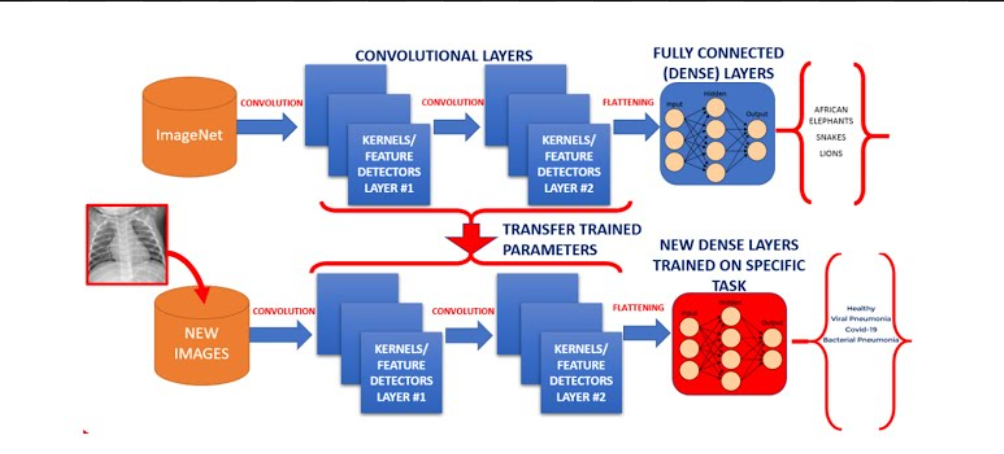
\includegraphics[width=0.8\textwidth]{images/Transfer-learning}
    \caption{Treniranje pomoću \emph{transfer learning-a}
    \protect\footnotemark}
    \label{fig:slika17}
\end{figure}
\FloatBarrier
\footnotetext{\url{https://www.coursera.org/projects/ai-powered-chest-disease-detection-and-classification}}

Transfer learning pruža nekoliko ključnih prednosti.
Prvo značajno ubrzava vrijeme treniranjam budući da model već posjeduje općenite značajke koje je prepoznao pri prvom treniranju.
Također, može značajno poboljšati performanse neuronske mreže, posebno kada imamo ograničeni skup podataka.
Taj dio je izuzetno važan jer za treniranje cijele mreže potrebna je velika količina podataka, a ona nekad jednostavno nije dostupna.

Važno je napomenuti da se, umjesto treniranje cijele mreže, često trenira samo dio nje, obično blizu izlaza.
To može uključivati dodavanje novih slojeva na kraj postojeće arhitekture ili treniranje samo izlaznog sloja s novim podatcima.
